%!TEX root = ../template.tex
%%%%%%%%%%%%%%%%%%%%%%%%%%%%%%%%%%%%%%%%%%%%%%%%%%%%%%%%%%%%%%%%%%%%
%% chapter4.tex
%% NOVA thesis document file
%%
%% Chapter with lots of dummy text
%%%%%%%%%%%%%%%%%%%%%%%%%%%%%%%%%%%%%%%%%%%%%%%%%%%%%%%%%%%%%%%%%%%%
\chapter{Approach and Planning}
\label{cha:approach_and_planning}

The work developed for this dissertation will start by collecting data from weather stations, soil sensors and farming fields(topology, geographic form, history of pest/disease). Integration with FitoAgro stations (WiseCrop \cite{wisecrop} and TerraPro \cite{terrapro}) will provide field variables. This means that, against the precision agriculture methodology refered in \ref{sec:precision_agriculture}, it will be assumed that the measurements made by a single point in the field are constant throughout the entire field. If some farming fields have no weather stations, the possibility of combining free satellite data (low temporal and geospatial resolution) is going to be analised. 

The figure \ref{fig:vis_pers_lowlevel} shows an example of a farming field visualization with low level of detail. 

\begin{figure}[htbp]
  \centering
  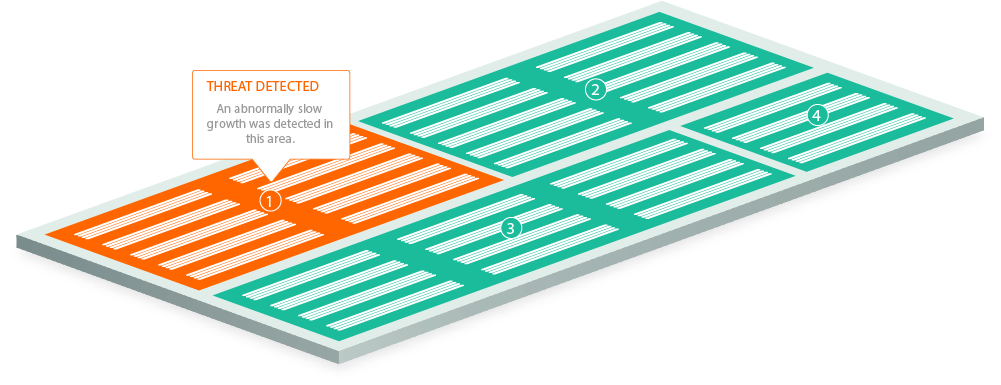
\includegraphics[width=0.7\linewidth]{vis_pers_lowlevel}
  \caption{Visualization of a farming field with a second level of detail: Plot.}
  \label{fig:vis_pers_lowlevel}
\end{figure}

The FitoAgro project is planned to be 4 years long. If during the first year (the time of development of the dissertation) the pest monitoring system evolves in terms of automation, efforts to gather more information will be made. This can mean paid satellite services (\textit{WorldView-3}) for intra-field data collection or soil sensors collecting ground information as of described in \ref{sec:soil_station}. Satellite data would mean getting crop growth levels, nutrients, soil moisture without having to install any sensors, but paying a fixed fee per hectare. Economic viability will be fully studied.

The only source that is to be collected at plant-level (measurements by tree), on this first stage of the project, are pest biological observations. Examples of visualization developed for the FitoAgro project in figures \ref{fig:vis_pers_highlevel} and \ref{fig:vis_2d_highlevel}.

\begin{figure}[htbp]
  \centering
  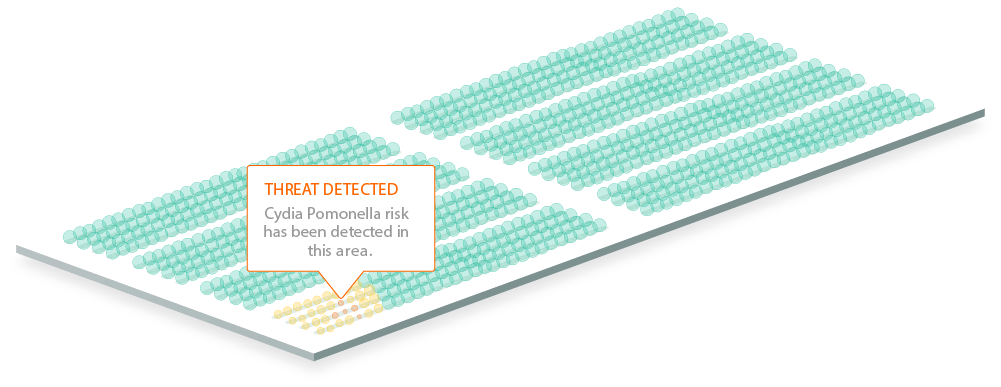
\includegraphics[width=1\linewidth]{vis_pers_highlevel}
  \caption{3D Visualization work for the FitoAgro project under development.}
  \label{fig:vis_pers_highlevel}
\end{figure}


\begin{figure}[htbp]
  \centering
  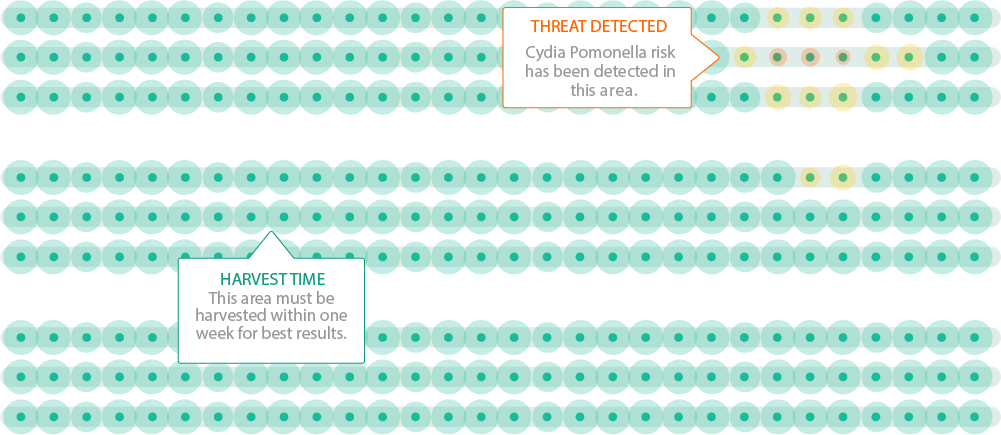
\includegraphics[width=0.6\linewidth]{vis_2d_highlevel}
  \caption{2D Visualization work for the FitoAgro project under development.}
  \label{fig:vis_2d_highlevel}
\end{figure}

These should present a good starting point for both the mobile and web interfaces (assuming 2D for smaller devices and 3D for laptop/desktop). When biological measurements are being performed, geolocation of the device should be taken into account to sucessfully map the measurement taken to a specific point in the field (therefore, tree being monitored).

The pest monitoring protocol is going to be closely followed \textit{in situ} to sucessfully iterate the proposed framework as in an agile methodology. Small development cycles should be made and testing on the fields as features are released. The interface will be tested directly with the users in a task-based test so see if the user is able to perform the directed task or not.

Since two members of the FCT-UNL institution are part of the FitoAgro project and dissertation topics shall not overlap, the server processing of this data is not mentioned in this work. Data collection is, ultimately, a server routine but also an important part of the work described in this very document. This being said, this work is being closely integrated to the work on \emph{André Malafaia}'s dissertation and the technological stack is going to be decided by both during the first days of dissertation work.

On enemy tracking, an event registering interface is going to be developed to be used directly in the field when registering biological observations. An example of the spreadsheet currently in use by the FitoAgro project managers and farmers can be found in \ref{fig:spreadsheet}. 